% !TEX encoding = UTF-8 Unicode

\section{Tradução de estruturas de controle de fluxo}

Será apresentado nas próximas seções, as traduções das estruturas de controle de fluxo que constam na nossa linguagem e foram solicitadas para essa entrega, entre elas as estruturas if, if-else e while.

Cabe ressaltar que foram utilizadas simbologias nas traduções que serão substituídas pelo compilador no momento da geração de código. Uma dessas marcações é os dois pontos no começo de uma linha que significa que os comandos devem ser colocados no início do código gerado. Outra simbologia criada é da forma {XN}, onde X representa uma letra maiúscula qualquer e N é o índice da instância dentro do tipo de marcação X. As opções para X são as seguintes:

\begin{itemize}
	\item \verb={C0}, {C1}, ...=: Conjunto de comandos
	\item \verb={R0}, {R1}, ...=: Referência
	\item \verb={L0}, {L1}, ...=: Label ou rótulo de uma instrução criados
            e exportados pelo código 
\end{itemize}

Há também a marcação \verb={N}=, utilizada para denotar que a primeira instrução do código subsequente ao comando atual deve ser adicionada no lugar da marcação. Estamos considerando substituir sempre a marcação \verb={N}= por uma instrução simples que só sirva para simplificar, como por exemplo somar zero ao acumulador.

Conceitos da pilha aritmética são utilizados para o cálculo de expressões
booleanas, no \autoref{sec:expre} explicações mais detalhadas são apresentadas. 

\subsection{Estrutura de controle de fluxo: IF}
\label{sec:if}

\lstinputlisting[frame=single,numbers=left,breaklines=true,morekeywords={JP,JZ,JN,LV,LD,MM,SC,RS,HM,GD,PD,OS}]{precompiled/if.pre}

\subsection{Estrutura de controle de fluxo: IF-ELSE}
\label{sec:if-else}

\lstinputlisting[frame=single,numbers=left,breaklines=true,morekeywords={JP,JZ,JN,LV,LD,MM,SC,RS,HM,GD,PD,OS}]{precompiled/ifelse.pre}

\subsection{Estrutura de controle de fluxo: WHILE}
\label{sec:while}

\lstinputlisting[frame=single,numbers=left,breaklines=true,morekeywords={JP,JZ,JN,LV,LD,MM,SC,RS,HM,GD,PD,OS}]{precompiled/while.pre}


\section{Tradução de comandos imperativos}

Essa seção explica as traduções dos comandos imperativos que constam na nossa linguagem e foram solicitadas para essa entrega, entre os quais os comandos de atribuição de valor, leitura da entrada padrão, impressão na saída padrão e chamada de subrotinas, associado à definicão de novas subrotinas. As mesmas definições das marcações explicadas anteriormente são válidas para as traduções a seguir.

\subsection{Atribuição de valor}
\label{sec:atribuicao-valor}

\lstinputlisting[frame=single,numbers=left,breaklines=true,morekeywords={JP,JZ,JN,LV,LD,MM,SC,RS,HM,GD,PD,OS}]{precompiled/atribV.pre}

\subsection{Comando de leitura}
\label{sec:leitura}

\lstinputlisting[frame=single,numbers=left,breaklines=true,morekeywords={JP,JZ,JN,LV,LD,MM,SC,RS,HM,GD,PD,OS}]{precompiled/read.pre}

\subsection{Comando de impressão}
\label{sec:impressao}

\lstinputlisting[frame=single,numbers=left,breaklines=true,morekeywords={JP,JZ,JN,LV,LD,MM,SC,RS,HM,GD,PD,OS}]{precompiled/write.pre}

\subsection{Definição e chamada de subrotinas}
\label{sec:subrotinas}

No caso da definição de subrotinas, a tradução fica a seguinte: 

\lstinputlisting[frame=single,numbers=left,breaklines=true,morekeywords={JP,JZ,JN,LV,LD,MM,SC,RS,HM,GD,PD,OS}]{precompiled/function.pre}

Vale salientar que as funcoes que tratam a pilha de registro de ativação foram
modificadas completamente para integração mais transparente na implementacao da
função. 

Já quando é identificada a chamada de uma subrotina já declarada, a seguinte tradução é utilizada:

\lstinputlisting[frame=single,numbers=left,breaklines=true,morekeywords={JP,JZ,JN,LV,LD,MM,SC,RS,HM,GD,PD,OS}]{precompiled/call.pre}


\section{Cálculo de expressões aritméticas e booleanas}
\label{sec:expre}

Além do que foi solicitado como obrigatório para essa entrega, 
pensamos ser importante definir a forma como fizemos a implementação do 
cálculo de expressões para a geração de código de saída.

Como o professor Ricardo Rocha nos explicou, a MVN não tem uma implementação
real de pilha, porém consegue simular a existência de uma pilha com o uso de
indirecionamentos que definem cada uma das operações da pilha, como \emph{push}
e \emph{pop}. Baseado nesse conceito de código alinhavado, definimos diversas
funções auxiliares que realizam operações simples de forma independente. Essas
funções nos permitiram realizar o cálculo de expressões de maneira mais clara e
com menos erros.

Para explicar de forma mais detalhada o processo utilizado para calcular as
expressões, vamos supor que lemos uma expressão \verb=1 + 2 * 3=. A gramática
que já implementamos nas etapas anteriores cria uma árvore que já considera a
ordem de prioridade das operações, fazendo com que a multiplicação ocorra antes
da soma. Para esse caso, o código de máquina deve primeiro empilhar o 1, em
seguida o 2 e depois o 3. Ao notar que uma operação de multiplicação foi
finalizada, ele retira da pilha dois operandos, no caso o 2 e o 3, realizando a
multiplicação e retornando a pilha o resultado da operação, no caso 6. Em
seguida, é efetuada a operação de soma com os dois operandos que estão na
pilha, o 1 e o 6, adicionando novamente o resultado, 7, na pilha.

\begin{figure}[htbp]
    \centering
    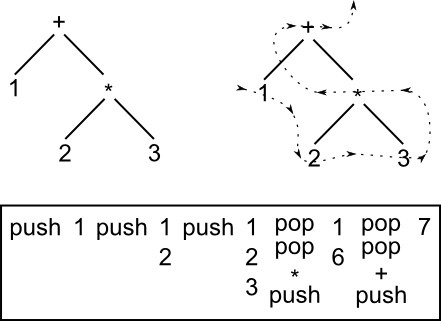
\includegraphics[width=.6\textwidth]{./img/arith.png}
    \caption{Árvore da expressão e operações resultantes na pilha.}
    \label{figure:example}
\end{figure}

O mesmo tipo de lógica foi implementado também para operadores booleanos e
permite a geração de código de forma mais simples, visto que já desenvolvemos
funções auxiliares para essas operações.

Apresentamos abaixo as operações principais da pilha aritmética. Todas as
outras operações da pilha se encontram no arquivo \verb!std.asm! no final do arquivo.


\begin{lstlisting}[frame=single,numbers=left,breaklines=true]
;--------------------------PUSH_ARITH------------------------------
PUSH_ARITH      JP /000
                MM TMP_1
                LD ARIT_PTR_STACK 
                +  TWO
                MM ARIT_PTR_STACK
                +  MOVE_CONST
                MM OP_PUSH_ARITH
                LD TMP_1
OP_PUSH_ARITH   JP /000 
                RS PUSH_ARITH 
;--------------------------POP_ARITH-------------------------------
POP_ARITH       JP /000 
                LD ARIT_PTR_STACK 
                -  TWO
                MM ARIT_PTR_STACK 
                +  TWO 
                +  LOAD_CONST 
                MM OP_POP_ARITH
OP_POP_ARITH    JP /000
                RS POP_ARITH 
;--------------------------SUM_ARITH-------------------------------
SUM_ARITH       JP /000 
                SC POP_ARITH
                MM TMP_2 
                SC POP_ARITH
                +  TMP_2 
                SC PUSH_ARITH
                RS SUM_ARITH 
;--------------------------MUL_ARITH-------------------------------
MUL_ARITH       JP /000 
                SC POP_ARITH
                MM TMP_2 
                SC POP_ARITH 
                *  TMP_2 
                SC PUSH_ARITH
                RS MUL_ARITH 
\end{lstlisting}


\section{Arrays e Structs}

Em \emph{CZAR} \textbf{não} existem \emph{Arrays} de tamanho dinâmico e sua criação está
limitada à declaração. Sendo assim, suas dimensões internas são conhecidas pelo
compilador a todo momento e seu cálculo de posição é facilitado e feito em
tempo de compilação. 

\begin{lstlisting}[frame=single,numbers=left,breaklines=true, language=C]
int i;

/* 
* Array int[4][3][2]: 
*
* [
*    [[0, 0], [0, 0], [0, 0]], 
*    [[0, 0], [0, 0], [0, 0]], 
*    [[0, 0], [0, 0], [0, 0]], 
*    [[0, 0], [0, 0], [0, 0]]
* ]
*
* Preenchendo com:
* ----------------
* decl int i;
* decl int j;
* decl int k;
* decl int l; 
* set i = 0;
* set j = 0;
* while (j < 4) {
*   set k = 0;
*   while (k < 3) {
*     set l = 0;
*     while (l < 2) {
*       set array_ex[j][k][l] = i;
*       set i = i + 1;
*       set l = l + 1;
*     }
*     set k = k + 1;
*   }
*   set j = j + 1;
* }
*
* Temos:
* ------
* [
*    [[0, 1], [2, 3], [4, 5]], 
*    [[6, 7], [8, 9], [10, 11]], 
*    [[12, 13], [14, 15], [16, 17]], 
*    [[18, 19], [20, 21], [22, 23]]
* ]
* ou:
* ---
* [
*   0, 1, 2, 3, 4, 5, 6, 7, 8, 9, 10,
*   10, 11, 12, 13, 14, 15, 16, 17, 18, 
*   19, 20, 21, 22, 23
* ]
*
*
*
*
*/
acc = acumulado[n_dimensoes - 1] = 1; // maybe long 1L 
for (i = n_dimensoes-2; i >= 0; i--) {
   acc = acumulado[i+1] = dimensoes[i+1] * acc;
}
/* 
   acumulado = [6, 2, 1];
*/
for (i = 0; i < n_dimensoes; i++) {
    acumulado[i] = acumulado[i] * size_cell; // celulas podem ter 
                                             // tamanho variavel
}
for (i = 0; i < n_dimensoes; i++) {
    fprints(str, " LV =%d ", acumulado[i]);
    cpy_to_lines_of_code(str);
    fprints(str, " * ARR_DIM_%d", acumulado[i]);
    cpy_to_lines_of_code(str);
    fprints(str, " +  ADDRS_ACCUMULATOR");
    cpy_to_lines_of_code(str);
    fprints(str, " MM ADDRS_ACCUMULATOR");
    cpy_to_lines_of_code(str);
}
\end{lstlisting}

O cálculo de \emph{structs} é resolvido em tempo de compilação. Uma vez que o
tamanho de cada parte da estrutura é conhecida em tempo de compilação, é
possível se fazer toda a aritmética de acesso via programação em \emph{C}. 

\begin{lstlisting}[frame=single,numbers=left,breaklines=true, language=C]
    int deslocamento_para_celula(struct_struct* vi_struct, int cell_to_access) {
        int sum_up_to_ptr = 0;
        for (i = 0; i < cell_to_access; i++) {
            sum_up_to_ptr += vi_struct->sizes[i];
        }
        return sum_up_to_ptr;
    }
\end{lstlisting}
